
\chapter{ Spécification et analyse des besoins}
%\tableofcontents

\textbf{\huge Introduction}\\[0.5cm] 

L'objectif de l'étape de spécification et d'analyse des besoins est de déterminer les fonctionnalités différentes attendues du système. Au cours de ce chapitre, nous présentons d'abord les acteurs concernés dans notre système. Ensuite, nous allons illustrer les besoins fonctionnels et non fonctionnels. Ensuite nous allons détailler le product backlog de notre projet. Ces exigences seront exprimées enfin sous forme de diagramme de cas d'utilisation qui sera détaillé par des scénarios possibles.
\section{\LARGE Acteurs}
\texttt{}\\[0.1cm]
 En génie logiciel et plus particulièrement en UML, un acteur est une entité qui définit le rôle joué par un utilisateur ou par un système qui interagit avec le système modélisé\cite{12}.\\\texttt{}\\[0.01cm]%add url
 \textsf{\fontfamily{ptm}\selectfont\scalefont{1.3}--Développeur :}C'est l'utilisateur qui peut modifier le code source d'un objectif donné (ajouter une fonctionnalité, corriger l'erreur, etc.) puis les déposer dans Github et ensuite suivre la compilation de l'application.\\\texttt{}\\[0.01cm]
\textsf{\fontfamily{ptm}\selectfont\scalefont{1.3}-- Ingénieur DevOps:} Est considéré comme l'acteur principal, son rôle est la mise en place du cluster, pipeline, surveiller l'état du système et configurer son infrastructure.\\\texttt{}\\[0.01cm]
\textsf{\fontfamily{ptm}\selectfont\scalefont{1.3}-- Client:} C'est l'utilisateur qui peut accéder à l'application déployée sur le cluster au moyen d'un site Web.\\\texttt{}\\[0.01cm]


\section{\LARGE Besoins fonctionnels}
\texttt{}\\[0.1cm]
 Pour le bon fonctionnement de notre projet, il est nécessaire de définir  concrètement les fonctionnalités qui seront implémentées dans le but de les rendre plus appropriées aux besoins de l'entreprise.
Pour cela nous avons allons présenter les besoins fonctionnels de notre projet:\\\texttt{}\\[0.01cm]
-- Mettre en place une solution hybride qui permet à l'entreprise d'exécuter des applications localement tout en profitant des avantages des services cloud.\\\texttt{}\\[0.01cm]
– Orchestrer les conteneurs pour garantir une haute disponibilité pour le déploiement et l'exécution des applications.\\\texttt{}\\[0.01cm]
– Automatiser le processus de déploiement avec Ansible pour aider avec les charges de travail.\\\texttt{}\\[0.01cm]
– Surveiller l’état du déploiement.\\\texttt{}\\[0.01cm]
– Créer un répertoire pour toutes les images Docker dans ECR (Elastic Container Registry).\\\texttt{}\\[0.01cm]
-- Enregistrer les artefacts dans un répertoire Nexus.\\\texttt{}\\[0.01cm]
– Utiliser Prometheus et Grafana pour surveiller le cluster kubernetes.\\\texttt{}\\[0.01cm]
– Assurer la qualité de code source avec SonarQube.\\\texttt{}\\[0.01cm]
– Gérer automatique des étapes de déploiement de clusters.


\section{\LARGE Besoins non-fonctionnels}
\texttt{}\\[0.1cm]
 Les besoins non fonctionnels établissent toutes les conditions nécessaires au bon fonctionnement du système et à l'amélioration de la qualité des services. Et pour répondre aux exigences fonctionnelles, notre projet doit respecter une série de propriétés contribuant à une meilleure qualité de la solution obtenue.
Nous déterminerons l'ensemble des contraintes à respecter pour garantir le bon déroulement du projet. Parmi les critères nous citons :\\\texttt{}\\[0.01cm]
--Confidentialité: Notre solution permettra de garantir la sécurité des données, des applications et des utilisateurs.\\\texttt{}\\[0.01cm]
--Performance: Rapidité du déploiement d'application sur des pods kubernetes et assurer la bonne exécution de ses applications.\\texttt{}\\[0.01cm]
--Disponibilité: Les clusters Kubernetes sont conçus pour permettre une évolutivité horizontale, ce qui signifie que les applications peuvent être déployées sur plusieurs nœuds et gérer de manière dynamique les charges de travail en fonction des besoins.\\\texttt{}\\[0.01cm]
--Maintenance: La modification d'un déploiement dans un kubernetes cluster doit être facilement maintenable et adaptable à de nouvelles exigences de sorte qu'il peut y avoir un changement ou l'ajout de nouvelle fonctionnalité.\\\texttt{}\\[0.01cm]
--Portabilité: Le système doit être flexible et capable de prendre en charge de nouvelles fonctions et extensions et doit pouvoir fonctionner avec un nouveau composant (RAM,stockage) et avec une modification minimale.\\\texttt{}\\[0.01cm]
--Extensibilité: Le système doit maintenir ses hautes performances sous pression et ajuster ses paramètres pour répondre à la demande, possibilité d’ajouter des nœuds en cas de montée en charge. \\\texttt{}\\[0.01cm]

\section{\LARGE Product Backlog}

Product Backlog est une liste de toutes les tâches connues pour être traitées par le produit. Il s'agit de la seule source des besoins pour toute modification du produit. Les besoins sont précisés par les user stories. Un "user story" se présente sous la forme suivante (voir tableau 2.1): \\[0.1cm]

\begin{table}[H]
  \begin{center}
    \resizebox{1.1\textwidth}{!}{%
  \begin{tabular}{|c|c|c| p{5cm}|c|}
    \hline
    id & Theme & Acteur & Description & Priorité \\
    \hline
    id 1 & gérer code source & Développeur & Permet de déposer le code ou le récupérer  & élevée \\
    \hline
    id2 & Suivre build d'application & Développeur & Peut voir la compilation de l'application & élevée \\
    \hline
    id3 & analyser qualité de code & Ingénieur DEVOPS & Permet  d'analyser le code source d'un projet et de détecter les erreurs de qualité avec SonarQube . &  élevée \\
    \hline
    id 4  & gérer liste des images docker & Ingénieur DEVOPS &  Consiste à répertorier et organiser les images Docker qui ont été créées .&  élevée \\
    \hline
    id 5 & gérer les artefacts d'application & Ingénieur DEVOPS &  Consiste à stocker et à gérer les différents composants d'une application, les bibliothèques, les configurations, les scripts et autres ressources .&  élevée \\
    \hline
    id 6 & Configurer l'architecture cloud & Ingénieur DEVOPS & Consiste à concevoir et à déployer une infrastructure informatique dans le cloud, en utilisant des services cloud pour répondre aux besoins. &  élevée \\
    \hline
    id 7 & Configurer le pipline & Ingénieur DEVOPS &  Est un processus important pour automatiser le processus de développement, de test et de déploiement d'une application. &  élevée \\
    \hline
    id 8  & Surveiller l'etat du cluster & Ingénieur DEVOPS &  Surveille l'état de tous les nœuds dans le cluster pour s'assurer qu'ils sont en bon état de fonctionnement et qu'ils répondent aux demandes des applications. &  élevée \\
    \hline
    id 9 & gérer la configuration du deploiement & Ingénieur DEVOPS & Assure que les applications sont déployées de manière cohérente et fiable &  élevée \\
    \hline
    id 10 & acces a l'application deployée & Client & s'assure qu'elle est accessible uniquement par les utilisateurs autorisés. &  élevée \\
    \hline
  \end{tabular}%
    }
  \end{center}
  \caption{Tableau du Product Back-log}
  \end{table}
  \texttt{}\\[0.5cm]

%\section{\LARGE  Conception de système}
%\textsf{\fontfamily{qtm}\selectfont\scalefont{1.3}
%Dnas ce qui suit,nous allons présenter les différent diagrammes de conception. }//[0.2cm]
\section{\Large  Diagramme de cas d'utilisation Global}


Le diagramme de cas d'utilisation global est utilisé pour une représentation du comportement fonctionnel d'un système logiciel.\\\texttt{}\\[0.01cm]
Le diagramme ci-dessous présente les cas d'utilisation généraux et les acteurs qui interagissent avec le système(Voir figure 2.1).
\begin{figure}[H]
  \begin{center}
  
      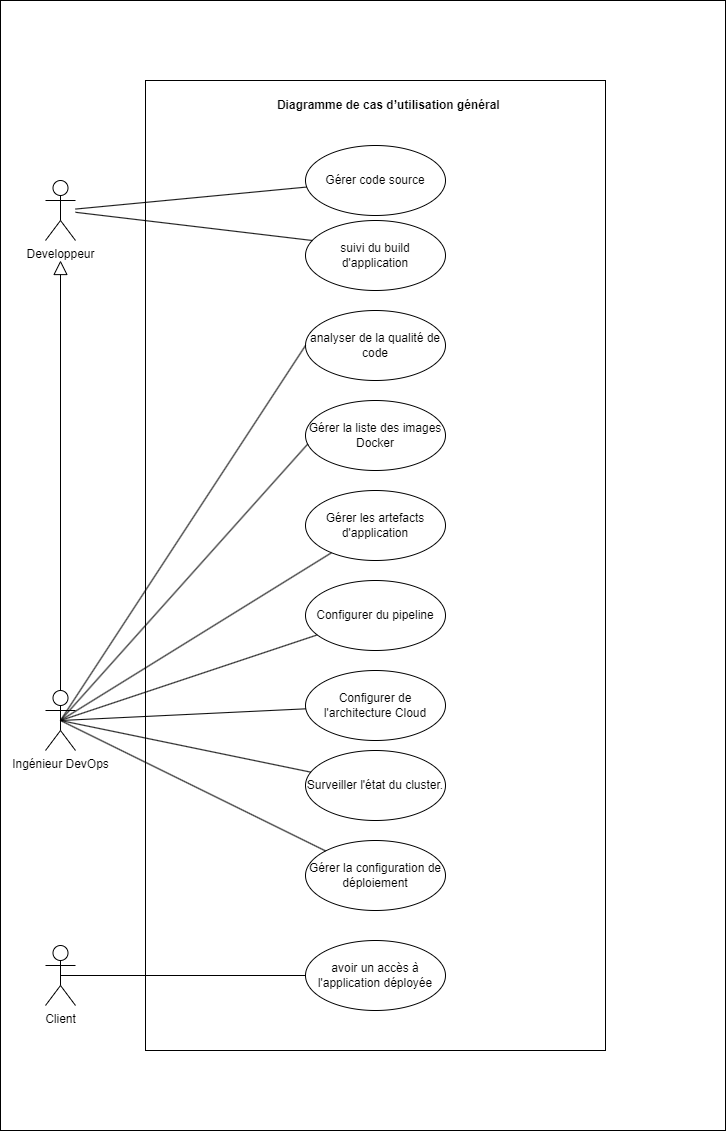
\includegraphics[width=12cm]{Use case.drawio.png}

  \end{center}
  
  \caption{Diagramme de cas d'utilisation Globale}
\end{figure}


Dans ce qui suit , le raffinnement des différents cas d'utilisation.\\[0.2cm]
\subsection{\Large Cas d’utilisation "Gérer code source"}
Dans cette section, nous décrirons de façon détaillée ce cas d'utilisation.\\\texttt{}\\[0.01cm]

\begin{figure}[H]
  \begin{center}
  
      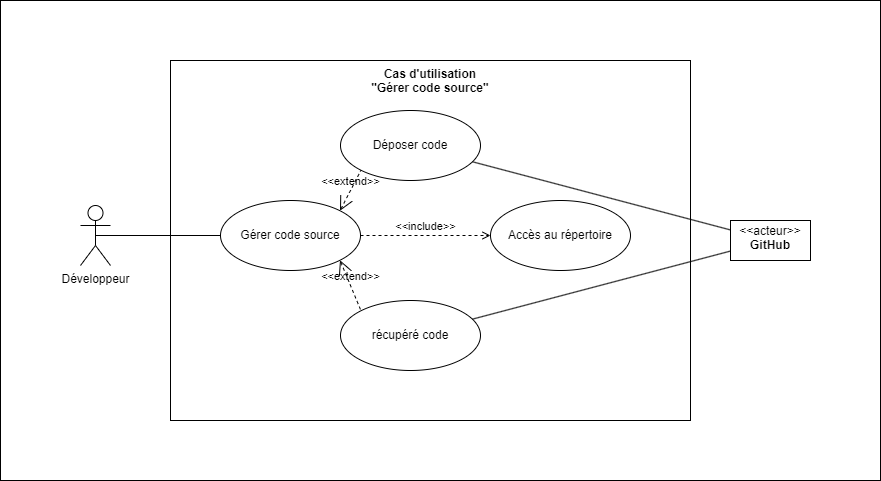
\includegraphics[width=15cm]{usecase1.drawio.png}

  \end{center}
  
  \caption{Cas d'utilisation:Gérer code source }
\end{figure}

Pour expliquer  le diagramme de cas d’utilisation, nous représentons la description textuelle du principales fonctionnalités mentionnées ci-dessus (Voir tableau 2.2): \\

\begin{center}
 \begin{table}[H] 
 \centering
 \resizebox{1.1\textwidth}{!}{%
 \begin{tabular}{|c|p{13cm}|}
 \hline
 Titre & Gérer code source\\
 \hline
 Acteur & Développeur \\
 \hline
 Description & le développeur peut déposer ou récupérer le code à travers le command "pull" ou "push".\\
 \hline
 Pré conditions & Une connexion établie entre le PC du développeur et le répertoire Git de l'application. \\
 \hline
 Post conditions & Code envoyé au répertoire git. \\
 \hline 
 \multirow{3}{*}{Scénario nominal} & 1- Avoir un accès au répertoire. \\
 & 2 - Gérer code source. \\
 & 3 - Déposer ou récuperer  le code dans le répertoire github. \\
 \hline
 \multirow{3}{*}{Scénario alternatif} & 1- La connexion entre la machine du développeur et Git ne peut pas être établie. \\
 & 2 - Le code ne peut pas être envoyé. \\
 & 3 - Retour à l'étape 1 du Scénario nominal. \\ 
 \hline
 \end{tabular}%
 }
 \caption{Description de cas d’utilisation:Gérer code source}
 \end{table}
\end{center}


   \subsection{\Large Cas d’utilisation "Suivi de la build d'application"}

Dans cette section, nous décrirons de façon détaillée ce cas d'utilisation.\\\texttt{}\\[0.01cm]

\begin{figure}[H]
  \begin{center}
  
      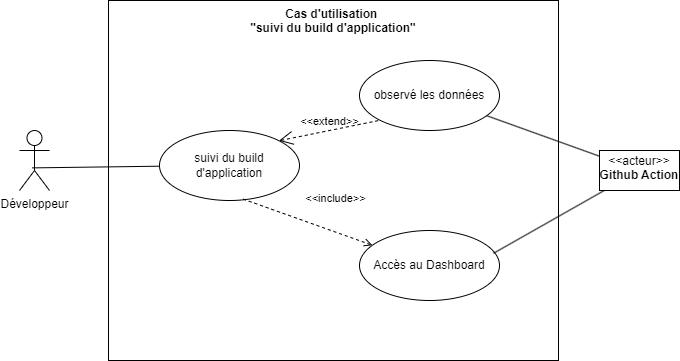
\includegraphics[width=15cm]{UseCase2.drawio.png}

  \end{center}
  
  \caption{Cas d'utilisation:Suivi la build d'application }
\end{figure}

Pour expliquer  le diagramme de cas d’utilisation, nous représentons la description textuelle des principales fonctionnalités mentionnées ci-dessus(voir tableau 2.3 ) : \\
\begin{center}
   \begin{table}[H]  
     \centering
     \resizebox{1.1\textwidth}{!}{%
     \begin{tabular}{|c|p{13cm}|}
      \hline
      Titre &  Suivi du build de l'application\\
      \hline
      Acteur & Développeur \\
      \hline
      Description & Le développeur peut suive la construction d'application pour connaître si la modification ajoutée au code source est valide ou non.\\
      \hline
      Pré conditions & Une connexion  établie entre le développeur et Github actions. \\
      \hline
      Post conditions & Affichage de Dashboard Github Actions. \\
      \hline 
      \multirow{3}{*}{Scénario nominal} & 1- Avoir un accès au Dashbord \\ 
      & 2- Suivi du build de l'application \\
      & 3- L'observation de la construction de l'application rapporte un succès.\\
      \hline
      \multirow{2}{*}{Scénario alternatif} & 1 - La connexion entre développeur et Github Actions ne peut pas être établie. \\
      & 2 - Retour à l'étape 1 du Scénario nominal.\\ 
      \hline
      \end{tabular}%
     }
   \caption{Description de cas d’utilisation:Suivi du build de l'application}
   \end{table}
   \end{center}
   \subsection{\Large Cas d'utilisation"Gérer la configuration de déploiement"}
    Dans cette section, nous décrirons de façon détaillée ce cas d'utilisation(voir figure 2.4).\\\texttt{}\\[0.01cm]
   
   \begin{figure}[H]
    \begin{center}
    
        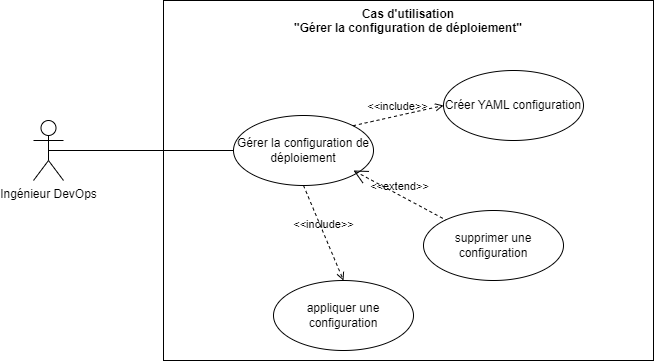
\includegraphics[width=15cm]{UserCase3.drawio.png}
  
    \end{center}
    
    \caption{Cas d'utilisation:Gérer la configuration de déploiement}
  \end{figure}
   
   Pour expliquer  le diagramme de cas d’utilisation, nous représentons la description textuelle des principales fonctionnalités mentionnées ci-dessus (voir table 2.4)  : \\
   \begin{center}
      \begin{table}[H]  
        \centering
        \resizebox{1.1\textwidth}{!}{%
        \begin{tabular}{|c|p{13cm}|}
         \hline
         Titre & Gérer la configuration de déploiement\\
         \hline
         Acteur & Ingénieur DevOps \\
         \hline
         Description & L'ingénieur DevOps gére la configuration de déploiement pour assurer la meilleure performance du cluster.\\
         \hline
         Pré conditions & Fonctionnement correct du cluster EKS. \\
         \hline
         Post conditions & Une configuration ou modification d'une configuration déjà existante. \\
         \hline 
        \multirow{2}{*}{Scénario nominal} & 1 - Lancer la configuration  du déploiement. \\
        & 2 - La configuration est lancée dans le contrôle plane d'EKS.\\
         \hline
        \multirow{3}{*}{Scénario alternatif} & 1 - La  nouvelle configuration n'est pas flexible. \\
        & 2 - Un problème apparaît causé par la nouvelle configuration.  \\
        & 3 - Retour à l'étape 1 du Scénario nominal.\\
         \hline
         \end{tabular}%
         }
      \caption{Description de cas d’utilisation:Gérer la configuration de déploiement}
      \end{table}
      \end{center}
      \subsubsection{\Large Cas utilisation"Gérer liste des images Docker"}
       
      Dans cette section, nous décrirons de façon détaillée le cas d'utilisation (voir figure 2.5).\\\texttt{}\\[0.01cm]
      
      \begin{figure}[H]
        \begin{center}
        
            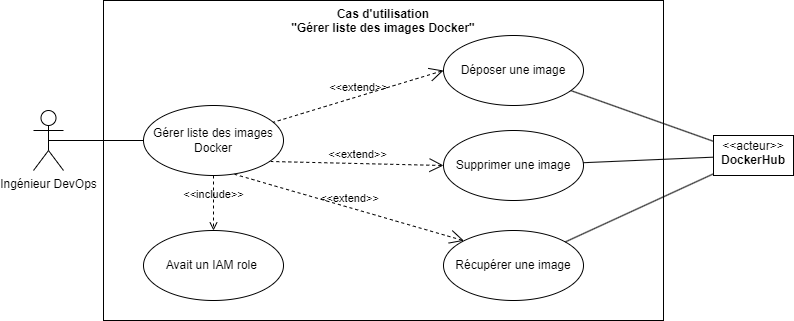
\includegraphics[width=15cm]{usecase5.drawio.png}
      
        \end{center}
        
        \caption{Cas d'utilisation:Gérer liste des images Docker}
      \end{figure}
      
      Pour expliquer  le diagramme de cas d’utilisation, nous représentons la description textuelle des principales fonctionnalités mentionnées ci-dessus (voir table 2.5) : \\
      \begin{center}
         \begin{table}[H]  
           \centering
           \resizebox{1.1\textwidth}{!}{%
           \begin{tabular}{|c|p{13cm}|}
            \hline
            Titre & Gérer liste des images Docker\\
            \hline
            Acteur & Ingénieur DevOps \\
            \hline
            Description & L'ingénieur DevOps gére la liste des images Docker\\
            \hline
            Pré conditions & Connexion au répertoire de l'application dans ECR. \\
            \hline
            Post conditions & Une image modifiée ,supprimée ou ajoutée. \\
            \hline 
           \multirow{4}{*}{Scénario nominal} & 1 - Se connecter ou l'enregistremementc de l'image n'est pas valide. \\
           & 2 -  Configurer liste des images Docker .\\
           & 2 - Déposer ou récuperer le code dans le répertoire ECR. \\
           & 3 - L'image est enregistrée dans la répertoire ECR.\\
            \hline
            \multirow{3}{*}{Scénario alternatif} & 1 - La connexion ou l'enregistrement de image n'est pas valide.  \\
            & 2 - Echec du dépose ou  récuperation l'image Docker .\\
            & 3 - Retour à l'étape 1 du Scénario nominal.\\
            \hline
            \end{tabular}%
           }
         \caption{Description de cas d’utilisation:Gérer liste des images Docker}
         \end{table}
         \end{center} 
         
      \subsection{\Large Cas utilisation"Gérer les artefacts d'application"}

         Dans cette section, nous décrirons de façon détaillée ce cas d'utilisation (voir figure 2.6).\\\texttt{}\\[0.01cm]
         
         \begin{figure}[H]
          \begin{center}
          
              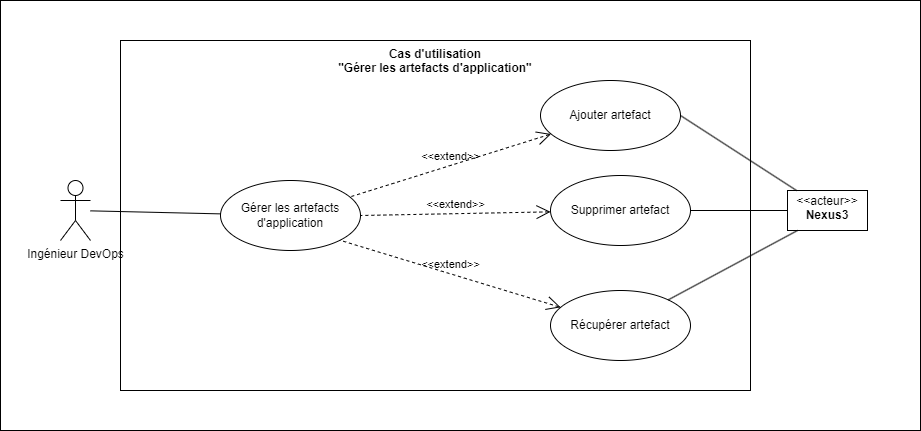
\includegraphics[width=15cm]{Usecase6.drawio.png}
        
          \end{center}
          
          \caption{Cas d'utilisation:Gérer les artefacts d'application}
        \end{figure}
         
         Pour expliquer  le diagramme de cas d’utilisation, nous représentons la description textuelle des principales fonctionnalités mentionnées ci-dessus ( voir table 2.6): \\
         \begin{center}
            \begin{table}[H]  
              \centering
              \resizebox{1.1\textwidth}{!}{%
              \begin{tabular}{|c|p{13cm}|}
               \hline
               Titre & Gérer les artefacts de l'application\\
               \hline
               Acteur & Ingénieur DevOps \\
               \hline
               Description & L'ingénieur DevOps gére la liste des artefacts pour assurer l'enregistrement de différentes versions d'application.\\
               \hline
               Pré conditions & Connexion HTTP au serveur Nexus. \\
               \hline
               Post conditions & Une répertoire avec les différentes artefacts de l'application.  \\
               \hline 
               \multirow{3}{*}{Scénario nominal} & 1 - Saisir les données d'authetification pour accéder à l'interface .\\
               & 2 - Configurer les artifacts d'application . \\
               & 3 - la connexion est réussite et la modification dans le répertoire est enregistrée dans Nexus .\\
               \hline
               \multirow{2}{*}{Scénario alternatif} & 1 - La connexion échoue ou la modification n'est pas enregistrée.  \\
               & 2 - Retour à l'étape 1 du Scénario nominal. \\
               \hline
               \end{tabular}%
              }
            \caption{Description de cas d’utilisation:Gérer les artefacts d'application}
            \end{table}
            \end{center}
\textbf{\huge Conclusion}\\[0.5cm] 

Dans ce chapitre nous avons décrit les différents besoins fonctionnels et non fonctionnels. Aussi, nous avons décrit les diffèrents acteurs de système.Puis nous avons présentée les "User stories" en forme d'un product backlog.Enfin, nous avons illustrée les cas d'utilisation avec des diagrammes. Dans le chapitre suivant nous passerons à la phase de conception du projet.


